\documentclass[11pt, a4paper]{article}

% --- Packages ---
\usepackage[utf8]{inputenc}
\usepackage[T1]{fontenc}
\usepackage{graphicx}
\usepackage{geometry}
\usepackage{siunitx}
\geometry{margin=1.75cm, headheight=26pt}
\usepackage{fancyhdr}
\usepackage{titlesec}
\usepackage{booktabs}
\usepackage{xcolor}
\usepackage{hyperref}
\usepackage{lastpage}

% --- ESA Official Colors (Approximate) ---
\definecolor{esablue}{RGB}{0, 50, 160}

% --- Hyperref Setup (Makes the ToC clickable) ---
\hypersetup{
  colorlinks=true,
  linkcolor=esablue,
  filecolor=magenta,      
  urlcolor=cyan,
}

% --- Section Numbering Tweaks ---
% This ensures sections are colored but keep their automatic numbering
\titleformat{\section}{\large\bfseries\color{esablue}}{\thesection}{1em}{}[\titlerule]
\titleformat{\subsection}{\bfseries\color{black}}{\thesubsection}{1em}{}

% --- Mission Metadata ---
\newcommand{\missionname}{Rømer I}
\newcommand{\missiontype}{Mission report}
\newcommand{\commander}{Adrian Fluturel}
\newcommand{\launchdate}{No launch date set}

% --- Header and Footer Setup ---
\pagestyle{fancy}
\fancyhf{}
\lhead{
\includegraphics[height=1cm]{../../assets/esa_logo.png}}
\chead{\textbf{\missionname} \\ \small ESA Mission Report}
\rhead{\missiontype}
\lfoot{Author: \commander}
\rfoot{Page \thepage\ of \pageref{LastPage}}
\renewcommand{\headrulewidth}{0.4pt}
\renewcommand{\footrulewidth}{0.4pt}

% --- Title Section Formatting ---
\titleformat{\section}{\large\bfseries\color{esablue}}{}{0em}{}[\titlerule]

\begin{document}

% --- Front Page ---
\begin{titlepage}
  \centering
  \vspace*{2cm}
  
\includegraphics[width=0.4\textwidth]{../../assets/esa_logo.png}\\[2cm]
  {\Huge \textbf{MISSION REPORT}}\\[0.5cm]
  {\LARGE \missionname}\\[1.5cm]
  
  \begin{table}[h]
    \centering
    \begin{tabular}{ll}
      \textbf{Status:} & PLANNING \\
      \textbf{Launch Date:} & \launchdate \\
      \textbf{Operator:} & ESA \\
      \textbf{Target:} & Mun \\
    \end{tabular}
  \end{table}
  
  \vfill
  \begin{center}
    \textit{This document contains technical specifications and
      trajectory plans for the \missionname\ mission as part of the Kerbin Expansion Initiative.}
  \end{center}
  \vfill
  
  {\large \today}
\end{titlepage}
  
% --- Table of Contents ---
\newpage
\renewcommand{\contentsname}{Mission directory}
\tableofcontents
\newpage

\section{Mission objectives}
The primary goal of the mission is to test the launch vehicle, the
cryogenic upperstage and the docking and life-support capabilities of
the LEM (Lunar Exploratory Module) and of the LCM (Lunar Command
Module).

The verification of the planned trajectory to the Mun, including the
ascent and the trans-lunar injection is also of importance. The crew
will be on a free-return trajectory, making sure that if anything will
happen to the service module, like a failed engine ignition, the crew
will still safely fall back down to Kerbin. For subsequent missions,
the plan is to put the vehicle on a free-return trajectory, and after
testing, the path will be modified to a prograde or retrograde
(depending on fuel margins) orbit around the Mun. This mission will
therefore also serve as practice for designing optimal free-returns.

Although landing on the Mun and the subsequent rendez-vous with the
LCM are planned for Rømer II, testing the parameters of the mission
and practicing the maneuvers needed for a successful landing and
eventual return to Kerbin is paramount.

\begin{figure}[h]
  \centering
  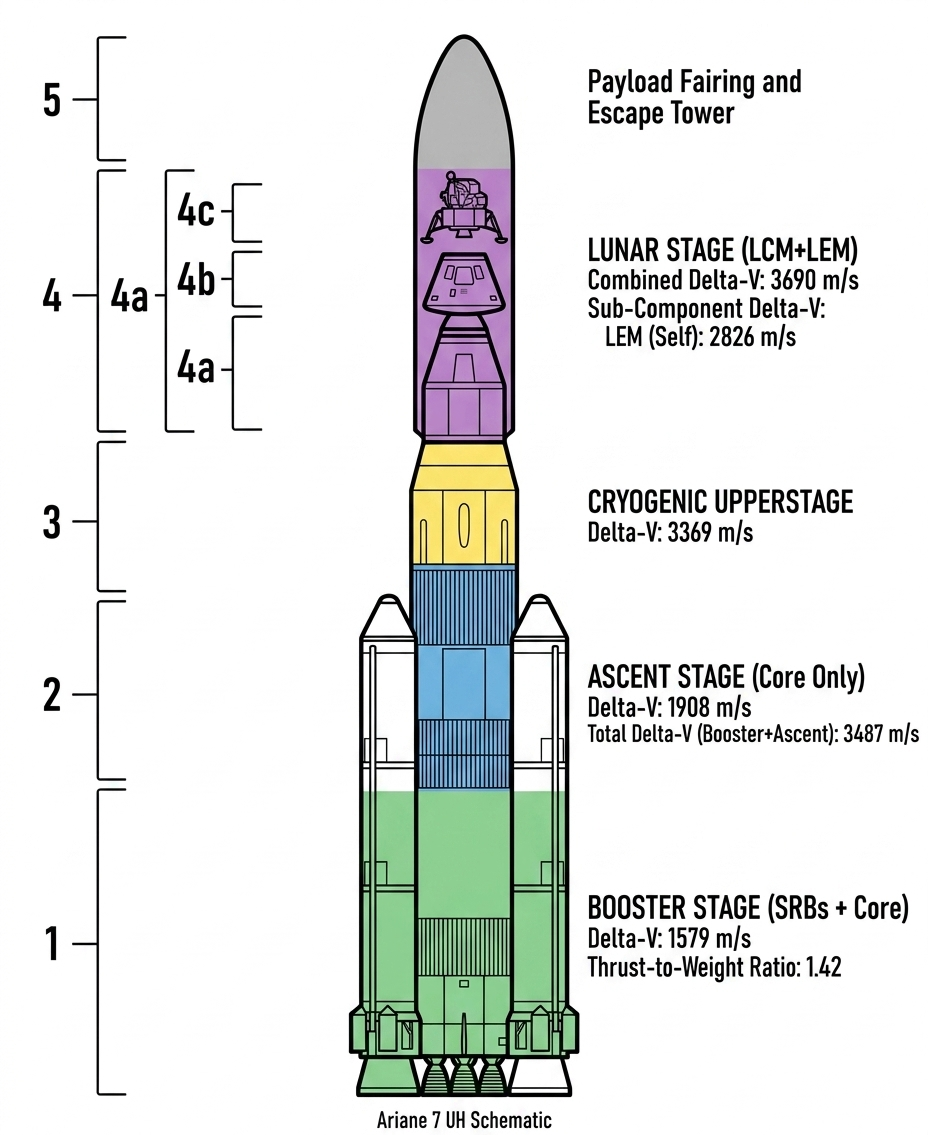
\includegraphics[width=0.7\textwidth]{../../assets/Mun/ariane7_uh.png}
  \caption{Schematic of the different stages and their associated
    performance numbers}
\end{figure}

\section{Vehicle specifications}
Presented next are the booster and the lander configurations used for
the mission. Some information is excluded here for the sake of brevity
but may be found in the description documents for the individual
parts, namely the booster and the LEM.

\subsection{Ariane 7 UH booster}
It is a standard Ariane 7 UH booster. The core stages are kept
intact. Even though the booster has addons for refueling in orbit and
airbrakes for landing, they were not removed in preparation for the
mission. The payload is the combined weight of the LEM, LCM, its
decoupling infrastructure and the fairing used to protect them during
ascent.

Below are the engineer readouts for the performance of the booster
given the payload present:
\begin{table}[h]
  \centering
  \caption{Ariane 7 UH Stage Specifications}
  \vspace{2mm}
  \begin{tabular}{l r r r r r r}
    \toprule
    \textbf{Stage} & \textbf{Body} & \textbf{Mass (t)} & \textbf{ISP (s)} & \textbf{Thrust (kN)} & \textbf{TWR (Max)} & \textbf{$\Delta v$ (m/s)}\\ 
    \midrule
    S3 & Mun & 43.243/71.977 & 350.0 & 250 & 5.06 (15.3) & 3690 \\
    S4 & Mun & 130.892/202.869 & 340.0 & 2,000 & 6.05 (16.62) & 3,369 \\
    S5 & Kerbin (Vac) & 294.839/497.708 & 305 & 4,050 & 0.83 (1.58) & 1,919 \\
    S6 & Kerbin (ASL) & 695.27/1,192.98 & 230.9 & 15,646.6 & 1.34 (2.73) & 1,615 \\ 
    \bottomrule
  \end{tabular}
\end{table}

A total of 10703 m/s (excluding the lander) was the total for this
payload. The capabilities of the lander were excluded from the table
(stages S0 through S2).

Stage S6 is the combined power of the first stage and the SRBs. It is
comprised of 3 liquid fuel engines (called the core stage) and 4 boosters. Its role is to get
the rocket through the thickest part of the atmosphere. Without the
SRBs, it is doubtful that the 3 liquid fuel engines alone would have
the TWR high enough to do that efficiently. Even though the engines
are optimized for sea-level pressure, their efficiency rises in the
upper parts of the atmosphere, increasing the $\Delta v$.

Once the side boosters are spent, the radial decouplers will
detach. That is stage S5. At that point, a good amount of fuel is left in the core
stage, but it is high enough in the atmosphere to be able to carry the
rest of the rocket on its own. Along with the radial decouplers, some
side-mounted separating boosters will push the SRBs safely away from
the main rocket. Now it's just the core stage until orbit.

After an expenditure of about 3600 m/s, the core stage is now empty
and it's detached as well. We enter stage S4, the cryogenic
upperstage. It is so called because it uses liquid oxygen and liquid
hydrogen as oxydizer and fuel respectively. This will give us the last
200 m/s necessarry to achieve a stable LKO (Low Kerbin Orbit). It
would also have enough fuel for the TLI, but that is withing the
purview of the LCM. The upperstage is equipped with remote control
computers. After separation, we deorbit the stage to remove space
clutter and debris. Optionally, if we choose to make an apoapsis raise
to conserver fuel before the TLI, this upperstage could be used for
that and discarded.

Finally, stage S4 is used for the TLI. Since we are planning a
free-return trajectory, no other burns except for course correction
are needed.

\begin{figure}[h]
  \centering
  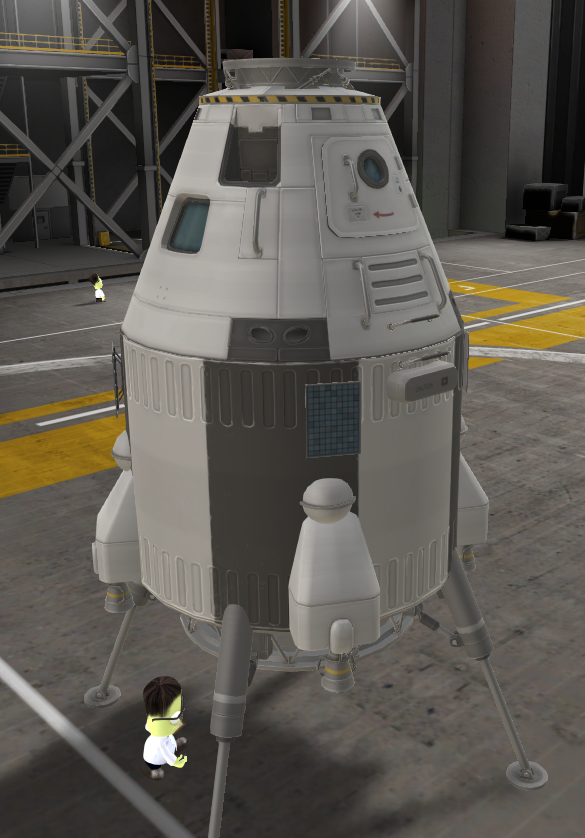
\includegraphics[width=0.3\textwidth]{../../assets/Mun/LEM.png}
  \caption{Picture of the LEM during construction}
\end{figure}

\subsection{Lunar Exploratory Module (LEM)}
The LEM is a light vehicle equipped with landing legs and enough fuel
to land from a circular low lunar orbit and achieve orbit from the
ground to rendez-vous with the LCM.

It is equipped with 4 Mk-1H Torch liquid engines and RCS
capabilities. The RCS was added so that the crew will be able to
control its attitude and make fine adjustments when docking with the LCM.

The MEL has no storage capacities, two solar pannel arrays
and 150 units of electricity. Electricity was not of major concern,
since the lander will never be piloted remotely. Of bigger concern was
the amount of monopropellant. Along with the built-in monopropellant
reserve next to the crew module, there are two more tanks of 7.5 units
attached radially.

It also presents with a Clamp-O-Tron docking port on the forward side
and LT-2 landing legs on the aft side. The landing legs are detachable
to save weight on the ascent from the Mun, but the reliability of the
decoupler is questionable and needs further study.

\begin{figure}[h]
  \centering
  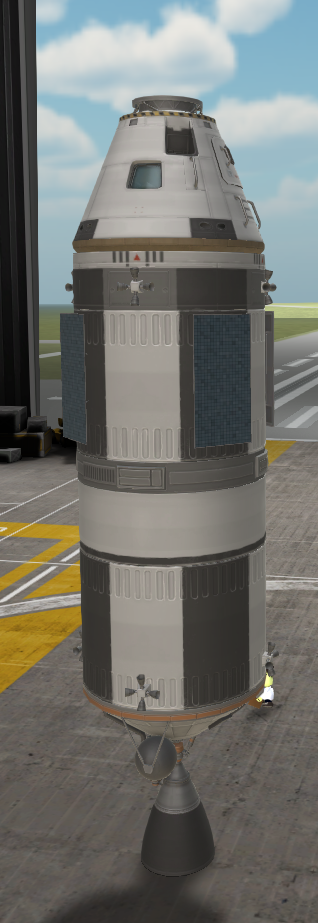
\includegraphics[width=0.3\textwidth]{../../assets/Mun/LCM.png}
  \caption{Picture of the LCM during construction}
\end{figure}

\subsection{Lunar Command Module (LCM)}
The LCM is where the crew will stay for the entirety of the mission,
except for some tests when in proximity with the moon. It is the main
operating grounds for maneuvers, communications and has the most
life-support. Unlike the LEM, there is more space and even a toilet in
the capsule.

The European Service Module is a subpart of the LCM, and is
responsible for controlling the engines, the RCS and the SAS
systems. After return to LKO and while on a trajectory to intercept
the atmosphere, the ESM will be discarded and it will safely burn up
in the atmosphere.

It has two deployable solar panel arrays and enough $\Delta v$ to
carry the LEM and the crew to the Mun and back.

\section{Crew}

As always, the crew requires at least a pilot and an engineer. A
scientist is preferred but not needed. A second pilot is also a
possibility. The crew will be limited to 3 people because of the Mk1-3
command pod used. Althought technically there are 2 such command pods
on the rocket assembly, one is for the lander and one is for the
command module. Upon docking during the trans-lunar trip, two kerbals
(a pilot and engineer) will transfer to the LEM to prepare it for the
landing procedure while the third crew member will stay in orbit with
LCM.

List of the chosen team members:
\begin{itemize}
\item{Hadbal Kerman} --- engineer and mission specialist
\item{Kerzer Kerman} --- pilot and LEM commander
\item{Malong Kerman} --- pilot and LCM commander
\end{itemize}

\section{Trajectory}

The trajectory poses multiple challenges from a mathematical
standpoint, chief of which is getting the correct injection angle into
the Mun's SOI. The ascent and the TLI itself are commonly done
maneuvers.

Additionally, fuel-saving measures will be taken to maximize
efficiency, although not strictly needed since the launch vehicle
(unmodified, which is not the case here since we removed stage S3) can
deliver approximately 305 tonnes to TLI, would be a good test to make
for future missions to optimize for fuel. These optimizations will
come in the form of splitting up expensive burns in multiple parts, as
needed.
\subsection{Ascent to LKO}
The ascent will be faily standard. Immediate after clearing the launch
tower, a roll program will be initiated to orient the rocket towards
heading \ang{90}. The roll should finish by the time the rocket hits
100 m/s going straight up. After that, a nominal pitch maneuever will
start executing to angle the rocket further east, at about \ang{20}
per minute. The actual pitch speed will depend on factors like drag
and time to apoapsis. It is preferable that the time to apoapsis stays
at about 1 minute throughout the gravity turn.

After 1 minute and 26 seconds, the SRBs will have finished their fuel
and will be detached from the main booster.

Nominal height at this point in the flight is approximately 20 km.

The core booster will continue burning for another 2 minutes and 54
seconds at full throttle. The actual time will depend on throttle
settings to keep the apoapsis time to 1 minute.

The desired parking orbit before other maneuvers is a circular
equatorial orbit of 75 kilometers. At that altitude, orbital speed is
given by the formula:

\[v = \sqrt{\mu \left(\frac{2}{75 + 600 km} - \frac{1}{75 + 600 km}
    \right)}\]
\[v = 2287 m/s\]

At an orbital speed of about 2.1 km/s, the core stage is separated. This
ensures the core stage will remain on a suborbital trajectory and burn
off in the atmosphere instead of being left in a stable orbit. The
remaining 100 m/s for circularization can be achieved with the
cryogenic upper stage.

\subsection{Apoapsis raise}

This is a fuel-saving technique and can therefore be omitted for the
TLI instead, but the exact phase angle and $\Delta v$ calculations
will be different.

The purpose of this maneuver is to take advantage of the Oberth effect
when raising the apoapsis for the Hohmann transfer to the Mun. Because
the orbit is circular and equatorial, the burn has the same fuel
requirements anywhere, but it should be \ang{180} from where the
desired apoapsis should be. The target orbit is an orbit with a period
of exactly 1 Kerbin sidereal day: 5h 59m 9.425s or 21549.425s.
The periapsis will necessarily remain at 75km. The apoapsis is
therefore found by calculating the semi-major axis of the target
orbit:
\[ T = 2pi \cdot \sqrt{\frac{a^3}{\mu}} \]
\[ a = \sqrt[3]{\frac{\mu \cdot T^2}{4\pi^2}} = \sqrt[3]{3.5316 \cdot 10^{12} \cdot \frac{21549.425^2}{4\pi^2}}\]
\[ a = \qty{3463334}{\metre}\]

Therefore, with a periapsis of 75 km, this results in an apoapsis of:
\[ r_a = 2a - r_p = \qty{6251.668}{\km} \]
\[ ap = r_{kerbin} - r_a = \qty{5651.668}{\km} \]

At periapsis, at this new target orbit, the speed should be:
\[ v_{periapsis} = \qty{3073.15}{\metre/\second}\]

Subtracting the previous value of \qty{2287}{\metre/\second},
this results in a prograde burn of \qty{786}{\metre/\second} to raise
the apoapsis.

The exact true anomaly at which we need to perform this burn will
depend on the location of the Mun. Since this is the first burn in a
two-burn maneuver that will result in the TLI, we need to make sure
that the Mun will be at the correct place when we perform our TLI
exactly one sidereal day from now.

That is, we need to calculate the phase angle between the ship and the
Mun knowing that in one sidereal day plus half of the orbital period
after the TLI burn, the phase angle will be a certain value. The exact
value will depend on how close we want to intersect the Mun.
\end{document}
